\documentclass[14pt,a4paper,oneside,fleqn,openright]{extbook}
\renewcommand{\baselinestretch}{1.50}\normalsize
\usepackage[top=3.5cm, bottom=3cm, left=3.5cm, right=2cm]{geometry}

\usepackage[utf8]{vietnam}
\usepackage{times}
\usepackage{graphicx}
\usepackage{datetime}

\usepackage{courier}
\usepackage{listings}
\lstset{
  basicstyle=\footnotesize\ttfamily,
  breaklines=true,
  frame=single,
  tabsize=2,
  showspaces=false,
  showtabs=false,
  tabsize=2,
  captionpos=b,
  columns=flexible
}
\renewcommand\lstlistingname{Mã nguồn}
\renewcommand\lstlistlistingname{Danh sách mã nguồn}
\def\lstlistingautorefname{Mã nguồn .}

\usepackage[nottoc,notbib]{tocbibind}
\usepackage[justification=centering]{caption}

\usepackage{lscape}
\usepackage{longtable}

\usepackage{fancyhdr}
\renewcommand{\headrulewidth}{0.5pt}
\renewcommand{\footrulewidth}{0.5pt}
%%% Header %%%
\fancyhead{}
\fancyhead[L]{\ifthenelse{\isodd{\value{page}}}{\it \nouppercase{\leftmark}}{\it \nouppercase{\rightmark}}}
\fancyhead[R]{\thepage}
%%% Footer %%%
\fancyfoot{}
\fancyfoot[L]{\ifthenelse{\isodd{\value{page}}}{\it Sinh viên: Dương Tiến Thuận - 50TH2}{\it Đồ án: Tiếp cận System Automation cho hạ tầng sản phẩm công nghệ}}

\usepackage[style]{fncychap}
\ChNameUpperCase
\ChNameVar{\raggedright \bfseries\normalsize}
\ChRuleWidth{1pt}
\ChTitleUpperCase
\ChNumVar{\raggedright\bfseries\normalsize}
\ChTitleVar{\raggedright\bfseries\Large}

\usepackage{hyperref}
\hypersetup{
  colorlinks        = true,
  bookmarksnumbered = true,
  allcolors         = blue,
  pdfauthor         = {Duong Tien Thuan - 50TH2 - 0851061294},
  pdftitle          = {TIEP CAN SYSTEM AUTOMATION CHO HA TANG SAN PHAM CONG NGHE},
  pdfsubject        = {ĐO AN TOT NGHIEP - CSE - WRU},
  pdfcreator        = {Thuan Duong <thuandt26@gmail.com>},
  pdfproducer       = {pdflatex},
  unicode           = true,
  pdffitwindow       = true,
}

\begin{document}

\author{Dương Tiến Thuận}
\title{Tiếp cận System Automation cho hạ tầng sản phẩm công nghệ}

\frontmatter
\pagestyle{empty}
\chapter*{\centerline{\bf \Large\MakeUppercase{Lời cảm ơn}}}
\addcontentsline{toc}{chapter}{Lời cảm ơn}

\vspace{20pt}

Trước khi trình bày nội dung chính của đồ án tốt nghiệp, em xin bày tỏ lòng
biết ơn sâu sắc tới Thạc sỹ Nguyễn Nam Hưng - người đã tận tình hướng dẫn, chỉ
bảo để em có thể hoàn thành đề tài này.

Em cũng xin bày tỏ lòng biết ơn chân thành tới toàn thể các thầy cô giáo trong
khoa Công Nghệ Thông Tin, Trường Đại học Thủy Lợi đã dạy bảo em tận tình trong
suốt quá trình học tập tại khoa.

Nhân dịp này em cũng xin được gửi lời cảm ơn chân thành tới gia đình, bạn bè đã
luôn bên em, cổ vũ, động viên, giúp đỡ em trong suốt quá trình học tập và thực
hiện đồ án tốt nghiệp.

\begin{flushright}
{\it Hà Nội, \today}

Sinh viên \hskip 2cm\quad

\vskip 2cm
{\bf Dương Tiến Thuận} \hskip 1cm \quad\
\end{flushright}

\thispagestyle{plain}

\newpage
\chapter*{\centerline{\bf \Large\MakeUppercase{Lời mở đầu}}}
\addcontentsline{toc}{chapter}{Lời mở đầu}

Điện toán đám mây\footnote{Cloud Computing: \url{https://en.wikipedia.org/wiki/Cloud_computing}} không còn là một khái niệm mới ở Việt Nam cũng như trên thế giới. Mặc dù điện toán đám mây chỉ là một cách khác để cung cấp các tài nguyên máy tính, chứ không phải là một công nghệ mới, nhưng nó đã châm ngòi một cuộc cách mạng trong cách cung cấp thông tin và dịch vụ của các doanh nghiệp - tổ chức trên toàn thế giới.

Sự phát triển nhanh chóng và mạnh mẽ của điện toán đám mây đã đặt ra nhiều thách thức đối với các nhà cung cấp dịch vụ (cloud providers) cũng như các doanh nghiệp, tổ chức sử dụng  nó. Áp lực đó không chỉ là cơ sở hạ tầng (hệ thống máy chủ, hệ thống mạng, trung tâm dữ liệu .v.v.) mà quan trọng hơn đó là yếu tố con người.

Đối với doanh nghiệp, điện đoán đám mây giúp giảm thiểu thời gian và chi phí đưa sản phẩm tới người dùng. Đối với quản trị hệ thống, điện toán đám mây mang lại khả năng mở rộng hệ thống một cách nhanh chóng, nhưng đồng thời nó cũng đặt ra thách thức trong việc quản lý hạ tầng máy chủ. Với số lượng hàng trăm server thì việc phải quản lý thủ công theo cách truyền thống là không hiệu quả và đem lại nguy cơ cao cho hệ thống. Từ yêu cầu thực tế đó, các framework cho việc tự động hóa hệ thống ra đời. Chúng cho phép người quản trị hệ thống có thể quản lý cấu hình của các máy chủ, đồng bộ hóa chúng với nhau, đồng thời đảm bảo việc nó không bị thay đổi sai bởi sự vô tình của con người. Không những thế, chúng còn cho phép người quản trị hệ thống triển khai ứng dụng một cách nhanh chóng tới nhiều môi trường và máy chủ khác nhau.

Các automation framework tiêu biểu được đề cập trong đồ án này bao gồm: Puppet, Chef và Ansible. Chúng đều là những sản phẩm mạnh mẽ và được sử dụng rộng rãi bởi nhiều doanh nghiệp, tổ chức lớn trên toàn thế giới.

Trong nội dung của đồ án này, em tập trung tìm hiểu cách sử dụng các automation framework và sau đó là ứng dụng chúng để tự động hóa các công việc liên quan đến hệ thống hạ tầng các sản phẩm công nghệ.

Hạ tầng sản phẩm công nghệ ở đây bao gồm:
\begin{itemize}
\item Hạ tầng máy chủ (Linux) cùng các cấu hình; các dịch vụ hệ thống như NTP, SSH, Cron, DHCP, DNS, .v.v.
\item Các dịch vụ và ứng dụng phục vụ trực tiếp cho sản phẩm như webserver (apache, nginx), database (postgresql, mysql) .v.v.
\end{itemize}

Việc phân chia 2 tầng như trên chỉ mang tính chất tương đối để chúng ta có thể xác định cụ thể quyền hạn và trách nhiệm của 2 dạng công cụ sẽ được đề cập đến trong đồ án là công cụ triển khai sản phẩm (deployment tool) và công cụ quản lý cấu hình (configuration manager).


\thispagestyle{plain}

\renewcommand{\baselinestretch}{1}\normalsize

%\setcounter{tocdepth}{4}
\tableofcontents
\listoffigures
\listoftables
\lstlistoflistings
\addcontentsline{toc}{chapter}{Danh sách mã nguồn}

\renewcommand{\baselinestretch}{1.50}\normalsize
\mainmatter
\pagestyle{fancy}
\newpage
\chapter{Tổng quan về tự động hóa hệ thống}
\newpage
\clearpage
\section{Lý do cần tự động hóa hệ thống}
Không phải ai cũng biết rằng, công việc của quản trị hệ thống thường xoay quanh một loạt các nhiệm vụ lặp đi lặp lại: cấu hình máy chủ, tạo người dùng, quản lý ứng dụng, dịch vụ và các chương trình chạy nền khác. Những công việc này thường được lặp đi lặp lại nhiều lần trong vòng đời của một máy chủ, từ lúc xây dựng hệ thống đến khi ngừng hoạt động. Nó bao gồm cả những việc như quản lý cấu hình trên nhiều cụm máy chủ khác nhau, đồng bộ hóa cấu hình giữa chúng theo chức năng; triển khai backend cho các sản phẩm; triển khai các sản phẩm trên các cụm máy chủ dịch vụ; dọn rác khi đĩa đầy, xóa log không dùng đến, xóa cache ... và đôi lúc là dọn "rác" của những người tiền nhiệm.

\newpage
\section{Các vấn đề nảy sinh}
\begin{itemize}
\item Quản trị hệ thống họ cũng là con người, họ có những vấn đề của con người\footnote{\url{http://en.wikipedia.org/wiki/Human_reliability}}. Điều nghiêm trọng nhất là quên và nhớ.

Một người quản trị hệ thống cho dù giỏi đến đâu cũng có sẽ có lúc quên chính xác những gì mình làm ở trong hệ thống của mình. Nhất là khi rất nhiều người cùng quản trị một hệ thống, mà hệ thống đó lại không được quản lý tốt. Đó là sẽ một vũng lầy!

\item Khi hệ thống đã là một vũng lầy, trên thực tế người ta sẽ đành chấp nhận nó. Nhưng sau một quá trình "chịu đựng", người ta sẽ tính đến chuyện đập đi làm lại, hay còn gọi là "migration". Cách giải quyết ở trong giai đoạn này thường chỉ mang tính chấp vá.

\end{itemize}


\newpage
\section{Cách giải quyết vấn đề}
\begin{itemize}
\item \textbf{Chuẩn hóa quy trình làm việc}

Điển hỉnh là các công ty Nhật, họ có một quy trình làm việc cực kì chặt chẽ, mọi thay đổi đều phải có quy trình và được kiểm soát nghiêm ngặt. Siết chặt các công đoạn làm việc, lịch sử thay đổi và công tác quản lý có thể sẽ hữu ích để giữ cho system không bị rối và luôn chạy ổn định.

\item \textbf{Chấp nhận sống trong "vũng lầy"}. 

Một điều đáng ngạc nhiên là có rất nhiều công ty, tập đoàn từ công nghệ đến cả tài chính trên thế giới phải làm kiểu này. Hệ thống vẫn hoạt động được và vẫn kiếm ra của cải, rất khó để có thể đưa một thay đổi đáng kể nào vào hệ thống đó. Người ta lúc này buộc lòng phải chấp nhận sống trong "vũng lầy"

\item \textbf{Tự động hóa hệ thống}

Đây là hướng mà đồ án này nói tới. Tuy việc tự động hóa hệ thống này đã được ứng dụng rộng rãi từ lâu nhưng nó vẫn là tập hợp của những công nghệ bleeding-edge\footnote{\url{http://en.wikipedia.org/wiki/Bleeding_edge_technology}}. Vì thế theo quan điểm của người viết đồ án thì nó chỉ phù hợp với các công ty công nghệ mà thôi.

\end{itemize}

\newpage
\section{Sự cần thiết của các công cụ quản lý}

Như đã nói ở trên, người quản trị hệ thống với những công việc lặp đi lặp lại này, điều thường thấy là người quản trị hệ thống sẽ cố gắng để tự động hóa chúng bằng các kịch bản (script) và các công cụ. Điều này dẫn đến sự phát triển của các ứng dụng và kịch bản tùy chỉnh. Những kịch bản này thường phức tạp, không có tài liệu đi kèm, và chỉ hoạt động trên một số hệ thống nhất định.

Việc này không có gì độc đáo cả, và việc phát triển các kịch bản này chỉ là một phản ứng thông thường với mong muốn làm cho công việc dễ dàng hơn, tự động hóa những việc thủ công nhàm chán để có thêm thời gian dành cho những điều thú vị hơn.

\begin{figure}[h!]
    \begin{center}
    \fbox{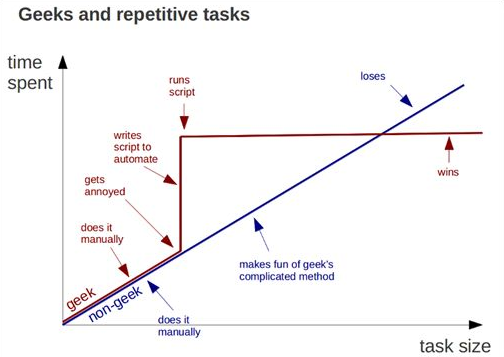
\includegraphics[width=0.9\textwidth]{images/Geeks_and_repetitive_tasks.png}}
    \end{center}
    \caption{Tự động hóa hệ thống bằng kịch bản}
    \label{fig:geeks_and_repetitive_tasks}
\end{figure}

Có rất ít các kịch bản đã được phát triển theo cách đặc biệt này được xuất bản, có tài liệu hay sử dụng lại. Thêm vào đó, bản quyền đối với hầu hết những kịch bản kể trên đều thuộc về những người quản trị hệ thống đã viết ra nó, và thường nó sẽ bị bỏ lại khi họ rời bỏ tổ chức đó hoặc chuyển sang vị trí khác. Điều này dẫn đến việc cùng một công cụ cứ được làm đi làm lại hết lần này đến lần khác. Thậm chí, đôi lúc chỉ đơn giản là điều đó không phù hợp với cách làm việc của người tại nhiệm hoặc người tại nhiệm không thể nắm bắt được những gì người tiền nhiệm đã để lại.

Khi hệ thống được mở rộng, những ứng dụng và kịch bản tùy chỉnh kiểu này hiếm khi phù hợp với môi trường lớn, và họ thường phải gặp phải rất nhiều vấn đề với tính ổn định, sự linh hoạt và các tính năng. Trong môi trường đa nền tảng, những kịch bản như vậy có xu hướng chỉ phù hợp với một nền tảng nhất định, dẫn đến trong các tính huống thực sự cần thiết sẽ phải tạo ra các kịch bản sử dụng cho BSD, một cái khác cho Linux và thậm chí là một cái khác nữa cho Solaris. Thật là tốn công sức và thời gian khi phát triển cũng như duy trì các công cụ như vậy với hy vọng nó sẽ giảm thiểu những công việc nhiêu khê mà bạn phải làm.

Một cách tiếp cận khác đó là mua các công cụ điều hành và quản lý cấu hình như Opsware của HP, CONTROL-M của BMC, Tivoli của IBM hay Unicenter của CA. Những công cụ thương mại này thường gặp phải 2 vấn đề chính đó là giá cả và tính linh hoạt. Đặc biệt là giá cả, nó có thể nhanh chóng trở thành một vấn đề lớn khi bạn sử dụng nhiều hơn các nền tảng và hạ tầng, giá có thể lên rất cao. Trong những hệ thống lớn, chi phí cho giấy phép sử dụng những công cụ như thế có thể lên tới hàng triệu USD.

Tính linh hoạt cũng là một mối quan tâm chính. Các công cụ thương mại thường đóng mã nguồn và giới hạn các tính năng có sẵn của chúng, có nghĩa là nếu bạn muốn mở rộng chúng để có thêm một tùy chỉnh nào đó phù hợp với hệ thống của bạn, bạn cần phải yêu cầu một tính năng mới, và đương nhiên nó có khả năng phải mất một thời gian chờ đợi và  một số khoản chi phí liên quan. Với sự đa dạng về việc triển khai, các nền tảng, các cấu hình và các ứng dụng trong các tổ chức, thật hiếm khi phát hiện bất kỳ công cụ cung cấp khả năng hoàn toàn tùy chỉnh cho phù hợp với môi trường của bạn.

Có một giải pháp thay thế cho cả việc phát triển phần mềm tự thân và phần mềm thương mại. Đó là Phần Mềm Tự Do Mã Nguồn Mở \footnote{Free and Open Source Software (FOSS): \url{https://en.wikipedia.org/wiki/FOSS}}. Các công cụ quản lý cấu hình mã nguồn mở cung cấp cho các tổ chức, doanh nghiệp 2 lợi ích chính sau:

\begin{itemize}
\item Chúng đi kèm mã nguồn nên có thể mở rộng được
\item Chúng là miễn phí!
\end{itemize}

Với các sản phẩm phần mềm nguồn mở, mã nguồn của công cụ trong tầm tay của bạn, cho phép bạn để phát triển cải tiến hoặc điều chỉnh của riêng bạn. Bạn không cần phải chờ đợi cho các nhà cung cấp để thực hiện các chức năng cần thiết hoặc trả tiền cho các tính năng mới hoặc thay đổi. Bạn cũng là một phần của một cộng đồng người sử dụng và phát triển những người chia sẻ một tầm nhìn cho sự phát triển của công cụ. Bạn và tổ chức của bạn có thể lần lượt đóng góp vào tầm nhìn đó. Kết hợp lại, bạn có thể định hình hướng đi của các công cụ bạn đang sử dụng, đem lại thêm sự linh hoạt tổ chức của bạn.

Bảng giá là một trong những yếu tố quan trọng đối với việc mua lại bất kỳ công cụ. Với phần mềm tự do mã nguồn mở, nó không phải là một vấn đề. Bạn không phải trả bất cứ gì cho phần mềm, và bạn sẽ có được mã nguồn với nó.

Tất nhiên, chúng ta đều biết chẳng bao giờ có một bữa ăn trưa miễn phí cả, vậy điều cần nắm bắt ở đây là gì? Không giống như phần mềm thương mại, phần mềm nguồn mở không đi kèm với bất kỳ sự hỗ trợ đảm bảo nào. Nói như thế không có nghĩa là sự hỗ trợ không có sẵn: Nhiều công cụ mã nguồn mở có cộng đồng lớn và rất năng động, ở đó các thành viên trả lời câu hỏi và cung cấp hỗ trợ thông qua các cơ chế như mailing list, diễn đàn, Wiki hay IRC.\footnote{Các công cụ mã nguồn mở, bao gồm cả Puppet hay Chef, cũng có tổ chức cung cấp các phiên bản thương mại hoặc hỗ trợ cho những công cụ này.}


\newpage
\chapter{Các công cụ tự động hóa hệ thống}
Trong chương trước, chúng ta đã đề cập tới sự cần thiết của việc sử dụng các công cụ quản lý cấu hình trong hế thống. Ở chương này chúng ta sẽ đi tìm hiểu một vài công cụ phổ biến trong việc quản lý cấu hình cũng như triển khai ứng dụng.

\newpage
\clearpage
\section{Puppet}
Puppet là một framework mã nguồn mở và là công cụ để quản lý cấu hình của hệ thống máy tính. Trong phần này, chúng ta sẽ tìm hiểu tổng quan về Puppet: cách thức nó hoạt động, cách nó quản lý cấu hình của hệ thống máy chủ, cách cài đặt chúng trên các nền tảng khác nhau. Tiếp đó, chúng ta sẽ tìm hiểu kiến trúc của Puppet, cách Puppet thu thập và quản lý các gói dữ liệu cấu hình.

\subsection{Tổng quan về Puppet}
Puppet là một công cụ quản lý cấu hình mã nguồn mở viết bằng Ruby, được sử dụng để quản lý cấu hình máy chủ và tự động hóa hệ thống trong các trung tâm dữ liệu của Google, Twitter, thị trường chứng khoán New York, và nhiều doanh nghiệp lớn khác. Puppet được phát triển đầu tiên bởi Puppet Labs, và hiện tại Puppet Labs cũng là người duy trì chính của dự án này. Puppet được dùng để quản lý có khi chỉ vài máy chủ nhưng cũng có khi lên tới 50.000 máy chủ, cùng với đó là đội quản trị hệ thống từ một người tới hàng trăm người.

Puppet là một công cụ để quản lý cấu hình và bảo trì hệ thống máy tính; ngôn ngữ cấu hình của nó rất đơn giản. Chúng ta chỉ cần chỉ cho Puppet thấy chúng ta muốn cấu hình máy tính của chúng ta như thế nào, nó sẽ thực hiện đúng những gì chúng ta muốn. Khi hệ thống có sự thay đổi chẳng hạn như một phiên bản cập nhật của gói phần mềm, thêm người dùng mới hay một cấu hình nào đó thay đổi, Puppet tự động cập nhật tất cả các máy chủ trong hệ thống đúng như cấu hình chúng ta muốn.

\begin{figure}[htb]
    \begin{center}
    \fbox{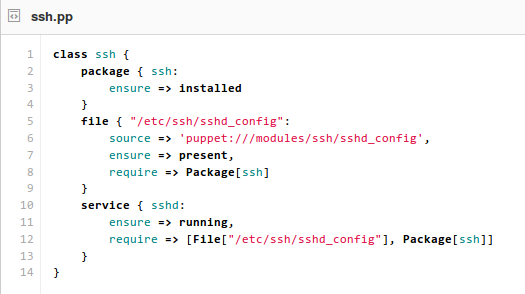
\includegraphics[width=0.9\textwidth]{images/puppet_ssh_pp.png}}
    \end{center}
    \caption{Ví dụ về ngôn ngữ cấu hình của Puppet}
    \label{fig:puppet_ssh_pp}
\end{figure}

Như hình vẽ trên, Puppet đảm bảo rằng gói phần mềm \textbf{\textit{ssh}} được cài đặt và file cấu hình dịch vụ SSH \footnote{Secure Shell: \url{https://en.wikipedia.org/wiki/Secure_Shell}} \textbf{\textit{/etc/ssh/sshd\_config}} của tất cả các máy chủ trong hệ thống mà Puppet quản lý đều có cùng nội dung mới file đã định trước; thêm vào đó, Puppet đảm bảo việc dịch vụ này luôn được chạy giúp người quản trị hệ thống có thể can thiệp thủ công khi cần thiết.

\subsection{Kiến trúc của Puppet}

Puppet được xây dựng với hai chế độ làm việc:

\begin{itemize}
\item \textbf{Chế độ client/server} Có một máy chủ trung tâm với một dịch vụ chạy nền kết nối đến các "agents" chạy độc lập trên các máy trạm.

\item \textbf{Chế độ serverless} Chỉ có một tiến trình duy nhất thực hiện tất cả các công việc.
\end{itemize}

Để đảm bảo tính nhất quán giữa các chế độ, Puppet luôn có sự minh bạch trong các liên kết nội bộ của bản thân nó. Do đó, hai chế độ này sử dụng cùng một đường dẫn như nhau cho dù chúng có giao tiếp với nhau qua mạng hay không. Mỗi lệnh được thực thi cho dù lấy cấu hình từ bản nó hay một máy khác ở xa trong mạng thì chúng đều có một cách thực hiện như nhau. Tuy nhiên cũng phải lưu ý rằng, chế độ serverless là một phần trong trong mô hình client/server: tất cả các file cấu hình sẽ được đẩy xuống cho agents ở máy trạm xử lý, tại đây máy trạm chạy ở chế độ serverless sẽ làm việc trực tiếp với các tệp tin cấu hình và thực thi chúng. Phần này sẽ chỉ tập trung vào chế độ client/server bởi vì nó dễ hiểu hơn với các thành phân riêng biệt, nhưng hãy luôn nhớ rằng tất cả đều chạy ở chế độ serverless.

Một trong những lựa chọn ngay từ đầu trong kiến trúc của Puppet là máy trạm không nên truy cập trực tiếp (raw access) vào các module, thay vào đó, chúng lấy các cấu hình đã được chuẩn bị sẵn từ trước. Việc này cung cấp nhiều lợi ích:

\begin{itemize}
\item \textbf{Thứ nhất}, chung ta thực hiện được việc tối thiểu quyền hạn cần thiết. Trong đó mỗi máy chủ chỉ biết chính xác những gì nó cần phải biết (nó nên được cấu hình như thế nào), nhưng nó không biết (và không quan tâm) những máy trạm khác được cấu hình như thế nào.

\item \textbf{Thứ hai}, chúng ta hoàn toàn có thể phân tách các quyền cần thiết để tạo ra một cấu hình (bao gồm cả quyền truy cập vào nơi lưu trữ dữ liệu trung tâm) mà nó sẽ được thực hiện dưới máy trạm.

\item \textbf{Thứ ba}, chúng ta có thể chạy các máy trạm trong chế độ ngắt kết nối với máy chủ trung tâm, nhưng các cấu hình đã có của Puppet sẽ vẫn luôn được áp dụng. Nghĩa là, cho dù máy chủ trung tâm (puppet-master) không còn hoạt động hoặc không có kết nối đến nó thì mỗi máy trạm vẫn có thể làm việc độc lập.

\end{itemize}

\begin{figure}[h!]
    \begin{center}
    \fbox{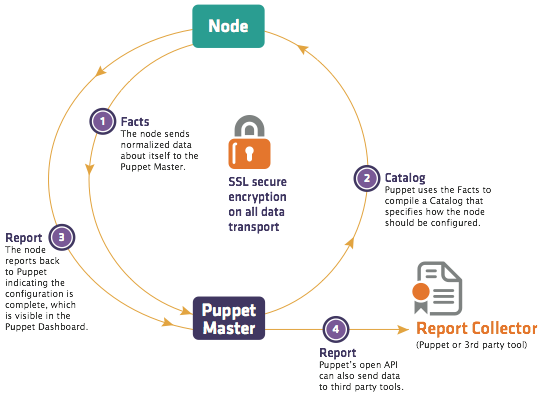
\includegraphics[width=0.9\textwidth]{images/puppet_dataflow.png}}
    \end{center}
    \caption{Biểu đồ luồng dữ liệu của Puppet}
    \label{fig:puppet_dataflow}
\end{figure}

Với sự lựa chọn này, quy trình làm việc trở nên tương đối đơn giản

\begin{itemize}
\item Tiến trình trên máy trạm (Puppet agent) thu thập các thông tin về hệ thống mà nó đang làm việc, sau đó chuyển các thông tin này tới máy chủ trung tâm (Puppet Master)

\item Tại máy chủ trung tâm, các thông tin đó cùng các module trên ổ đĩa cục bộ được biên dịch thành một cấu hình cho một máy chủ cụ thể và trả lại nó cho các tiến trình trên máy trạm.

\item Các tiến trình trên máy trạm áp dụng những cấu hình cục bộ này và nó chỉ ảnh hưởng tới riêng máy trạm đó. Sau đó, các tập tin báo cáo được tạo ra rồi đưa kết quả về máy chủ trung tâm.
\end{itemize}

Vì thế, các agent có quyền truy cập vào thông tin riêng trên hệ thống của mình, các cấu hình của nó, cũng như các báo cáo nó tạo ra. Máy chủ trung tâm có bảo sao của tất cả các dữ liệu này, cùng với quyền truy cập toàn bộ các module, cũng như bất kỳ cơ sở dữ liệu và dịch vụ nào khác dùng để biên dịch các cấu hình cần thiết.

\begin{figure}[h!]
    \begin{center}
    \fbox{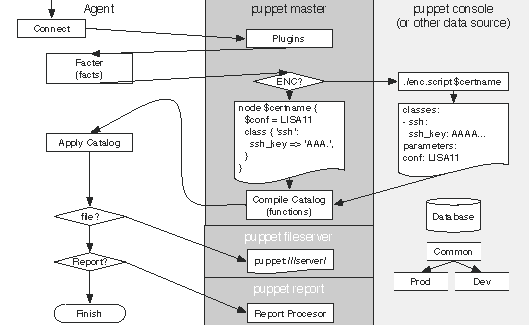
\includegraphics[width=0.9\textwidth]{images/puppet_timing_diagram.png}}
    \end{center}
    \caption{Luồng dữ liệu lưu chuyển \\ giữa các thành phần và tiến trình của Puppet}
    \label{fig:puppet_timing_diagram}
\end{figure}

Ngoài các thành phần ở trong quy trình làm việc này, có rất nhiều loại dữ liệu được Puppet sử dụng cho các giao tiếp nội bộ của nó. Các loại dữ liệu rất quan trọng, bởi vì chúng hoàn thực hiện tất cả các thông tin liên lạc, đồng thời chúng cũng cung cấp các giao diện công cộng cho những công cụ khác sử dụng hay làm việc với chúng.

\newpage
\clearpage
Các kiểu dữ liệu quan trọng nhất trong Puppet là:

\begin{itemize}
\item \textbf{Facts}: Thu thập các thông thin hệ thống trên mỗi máy trạm. Những thông tin này được dùng để biên dịch ra các cấu hình.

\item \textbf{Manifest}: Các tập tin chứa ngôn ngữ cấu hình Puppet, chúng thường được tổ chức thành các bộ sưu tập được gọi là module.

\item \textbf{Catalog}: Một đồ thị về các tài nguyên của máy chủ được quản lý và các rằng buộc giữa chúng.

\item \textbf{Report}: Tập hợp tất cả các sự kiện được tạo ra trong suốt quá trình tạo ra các Catalog.
\end{itemize}

Ngoài Facts, Manifests, Catalogs, and Reports, Puppet còn hỗ trợ các kiểu dữ liệu như các tệp tin, các chứng chỉ (được dùng trong việc xác thực) cùng nhiều kiểu dữ liệu khác.

\begin{figure}[h!]
    \begin{center}
    \fbox{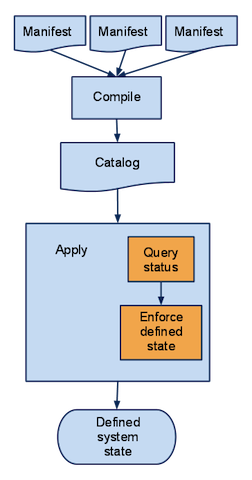
\includegraphics[scale=1.0]{images/puppet_manifest_to_defined_state_unified.png}}
    \end{center}
    \caption{Cách Puppet biên dịch và thực hiện một manifest\\ trong chế độ Serverless}
    \label{fig:puppet_manifest_to_defined_state_unified}
\end{figure}

\begin{figure}[h!]
    \begin{center}
    \fbox{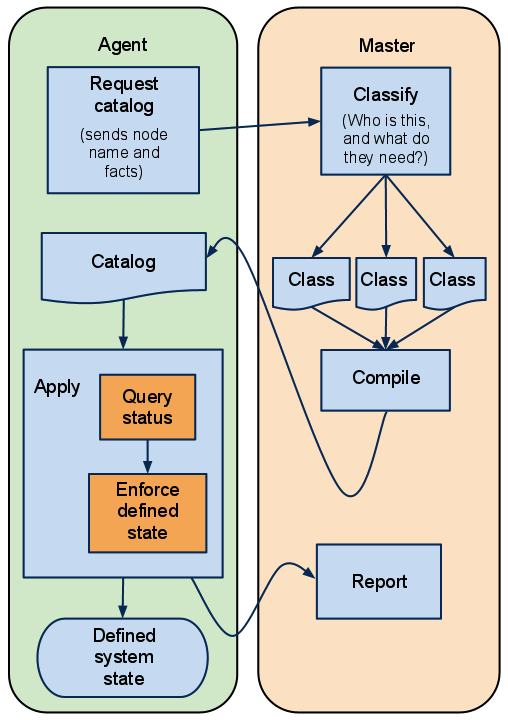
\includegraphics[width=0.85\textwidth]{images/puppet_manifest_to_defined_state_split.png}}
    \end{center}
    \caption{Cách Puppet biên dịch và thực hiện một manifest\\ trong chế độ Client-Server}
    \label{fig:puppet_manifest_to_defined_state_split}
\end{figure}

\clearpage
\subsection{Các thành phần của Puppet}
Các thành phần chính của Puppet bao gồm: Agent, Facter, ENC, Compiler, Transaction, RAL và Reporting


\textbf{\large Agent}


Thành phần đầu tiên mà chúng ta tiếp xúc khi sử dụng Puppet là tiến trình agent. Trong các phiên bản trước của puppet, tiến trình này được tách riêng thành một tiến trình riêng biệt có tên là \textbf{\textit{puppetd}}, nhưng trong phiên bản 2.6 trở đi, chúng được tối giản hóa và bây giờ chúng được gọi bằng lệnh \textbf{\textit{puppet agent}}, tương tự như cách làm của Git\footnote{Một hệ thống quản lý mã nguồn phân tán \url{http://git-scm.com/}}. Các agent thực hiện rất ít các chức năng của riêng nó mà chủ yếu các công việc liên quan đến các cấu hình hay mã nguồn được thực hiện ở phía máy trạm như trong quy trình làm việc đã mô tả ở trên.


\textbf{\large Facter}


Thành phần tiếp theo sau agent là một công cụ bên ngoài gọi là \textbf{\textbf{facter}}, đó là một công cụ đơn giản được sử dụng để tìm kiếm và thu thập các thông tin về hệ thống nó đang chạy trên đó. Thông tin đó thường là hệ điều hành, địa chỉ IP, tên máy chủ, nhưng vì Facter là một công cụ có khả năng mở rộng nên rất nhiều các tổ chức thường thêm vào các plugin riêng họ để thu thập các thông tin khác mà họ cần. Các agent gửi những thông tin mà Facter đã thu thập được tới máy chủ trung tâm, nơi nó được tiếp quản và xử lý theo quy trình ở hình \ref{fig:puppet_dataflow}


\textbf{\large External Node Classifier}


Trên máy chủ trung tâm, thành phần đầu tiên chúng ta cần đề cập tới là External Node Classifier\footnote{Các lớp phân loại mở rộng} hay ENC. ENC chấp nhận tên máy trạm hoặc trả về các cấu trúc dữ liệu đơn giản có chứa các cấu hình cấp cao của máy chủ đó. ENC nói chung là một ứng dụng hay dịch vụ riêng biệt: điển hình là một vài sản phẩm mã nguồn mở như Puppet Dashboard hay Foreman; đôi khi nó được tích hợp vào hệ thống dữ liệu có sẵn chẳng hạn như máy chủ LDAP... Mục đích cơ bản của ENC là để xác định những gì mà các lớp chức năng thuộc về, kèm theo đó là những thông số cấu hình cho các lớp này. Ví dụ, một máy trạm có thể thuộc lớp \textbf{\textit{debian}} hay \textbf{\textit{webserver}} và chúng có tham số để báo rằng chúng ở trung tâm dữ liệu tại \textbf{\textit{atlanta}}

Lưu ý rằng như Puppet 2.7, ENC không phải là một thành phần bắt buộc, thay vào đó người dùng có thể trực tiếp chỉ định cấu hình tại mỗi nút của Puppet. ENC được hỗ trợ trong khoảng 2 năm sau khi Puppet ra đời, bởi vì những nhà phát triển nhận ra rằng các lớp về cơ bản là khác biệt với các việc cấu hình chúng. Và, nó sẽ có ý nghĩa hơn nhiều khi đưa những vấn đề này vào các công cụ riêng biệt thay vì mở rộng ngôn ngữ để hỗ trợ cả hai cơ sở này. ENC luôn luôn khuyến khích sử dụng, và tại một số nơi nó trở thành một thành phần cần thiết (lúc này Puppet sẽ xuất hiện với tư cách một công cụ hữu ích hơn là một gánh nặng).

Một khi máy chủ trung tâm nhận được thông tin phân loại theo lớp từ ENC và thông tin hệ thống từ facter (thông qua các agent), nó đóng gói tất cả các thông tin vào một đối tượng Node và chuyển nó vào các trình biên dịch (Compiler).


\textbf{\large Compiler}


Như đã đề cập ở trên, Puppet có một ngôn ngữ tùy chỉnh được xây dựng dành riêng cho việc cấu hình hệ thống. Trình biên dịch này bao gồm 3 khối: một bộ phân tích ngôn kiểu-Yacc\footnote{https://en.wikipedia.org/wiki/Yacc} đã được tùy chỉnh; một nhóm các lớp học sử dụng để tạo ra Cây cú pháp trừu tượng (Abstract Syntax Tree hay AST); sau cùng lớp biên dịch, nó xử lý các tương tác của tất cả các lớp, đồng thời cũng có chức năng như API và là một phần của hệ thống.


\textbf{\large Transaction}


Khi các Catalog đã được xây dựng thành công, nó được chuyển qua cho lớp Transaction. Trong một hệ thống mà máy trạm và máy chủ trung tâm được tách biệt, bộ phận này được chạy trên máy trạm, nó có nhiệm vụ kéo xuống các Catalog qua giao thức HTTP như Hình \ref{fig:puppet_timing_diagram}.

Lớp Transaction thực hiện một công việc tương đối đơn giản: tìm sự rằng buộc trong các mối quan hệ và đảm bảo các tài nguyên đấy được đồng bộ. Nó thực hiện một quá trình với 3 bước đơn giản: lấy trạng thái hiện tại của tài nguyên đó, so sánh nó với trạng thái mong muốn và thực hiện bất kì thay đổi cần thiết nào để sữa chữa sai lệnh.


\textbf{\large Resource Abstraction Layer}


Như đã biết, lớp Transcaction là rất quan trọng sự hoàn thành các công việc trong Puppet, nhưng thật ra, tất cả các công việc được thực sự thực hiện bởi lớp tài nguyên trừu tượng (Resource Abstraction Layer, viết tắt là RAL). Đây cũng là một trong các thành phần thú vị nhất của Puppet.

RAL là thành phần đầu tiên được tạo ra trong Puppet, hơn cả ngôn ngữ cấu hình, nó định nghĩa rõ ràng những gì con người có thể làm với nó. Công việc của RAL là xác định những gì là tài nguyên và cách các tài nguyên đó có thể thực hiện công việc của nó trên hệ thống. Sau đó ngôn ngữ Puppet được cụ thể hóa thành các mô hình bằng RAL. Bởi vì điều này nên nó là thành phần quan trọng nhất trong hệ thống, và khó khăn nhất để thay đổi. Có rất nhiều điều những nhà phát triển muốn khắc phục trong RAL, và họ đã thực hiện rất nhiều cải tiến quan trọng đối với nó trong nhiều năm qua (quan trọng nhất là việc bổ sung các Providers ), nhưng vẫn có rất nhiều việc phải làm với RAL trong dài hạn.

Như đã nói, lớp Transaction không thực sự ảnh hưởng  trực tiếp đến hệ thống, mà nó dựa vào RAL để làm việc đó. Trong thực tế, providers là thành phần duy nhất của Puppet mà thực sự tác động vào hệ thống. Nếu lớp Transaction yêu cầu nội dung của một tập tin thì lớp Providers tìm kiếm và thu thập nó; nếu lớp Transaction xác định rằng nội dung của một tập tin nên được thay đổi thì lớp Providers sẽ thay đổi nó. Tuy nhiên phải lưu ý rằng, bản thân lớp Providers không bao giờ có quyền quyết định ảnh hưởng đến hệ thống mà chính lớp Transaction mới có quyền này, lớp Providers chỉ là người thực hiện công việc. Điều này cho phép các lớp Transaction kiểm soát hoàn toàn mà không yêu cầu phải hiểu bất cứ điều gì về các tập tin, người dùng, hoặc các gói. Sự phân chia rõ ràng này cho phép Puppet có sự mô phỏng đầy đủ nơi mà chúng ta có thể đảm bảo phần lớn hệ thống không bị ảnh hưởng.


\textbf{\large Reporting}


Trong quá trình lớp transaction đi theo các đồ thị và sử dụng RAL để thay đổi các cấu hình của hệ thống, các bản báo cáo được tạo ra. Báo cáo này bao gồm hầu hết cac sự kiện được tạo ra bởi những thay đổi trong hệ thống. Những sự kiện này, chúng là phản ảnh toàn diện về những công việc đã thực hiện: mốc thời gian thay đổi, giá trị trước đó, giá trị mới và bất kì thông báo nào được tạo ra, và tất nhiên là việc thay đổi đó thành công hay thất bại.

Các sự kiện được bao bọc trong một đối tượng ResourceStatus được ánh xạ vào từng tài nguyên. Vì vậy, đối với một giao dịch nhất định, chúng ta biết tất cả các nguồn tài nguyên đã được sử dụng, tất cả các thay đổi đã xảy ra, cùng với tất cả các metadata mà chúng ta cần biết về thay đổi đó.

Sau khi giao dịch hoàn tất, một số số liệu cơ bản được tính toán và lưu trữ trong báo cáo, và sau đó nó được gửi đến máy chủ trung tâm (nếu cấu hình). Với báo cáo đã gửi, quá trình cấu hình hoàn tất, các agent sẽ quay về trạng thái nghỉ hoặc là tự động kết thúc.


\subsection{Hệ thống hạ tầng của Puppet}

Trong mục này chúng ta sẽ tìm hiểu các thành phần hạ tầng của Puppet

\textbf{\large Hệ thống các Plugin}

Một trong những điều tuyệt vời của Puppet là nó có khả năng mở rộng rất tốt. Có ít nhất 12 loại mở rộng khác nhau của Puppet, có nghĩa nó có thể sư dụng cho bất kì ai. Ví dụ, chúng ta có thể bổ sung các tùy chỉnh trong các lĩnh vực sau:

\begin{itemize}
\item Các kiểu tài nguyên hay provider tùy chỉnh.
\item Cách xử lý các báo cáo cũng như việc lưu trữ các báo cáo này vào cơ sở dữ liệu riêng.
\item Bổ sung thêm các Indirector để tương tác với những cơ sở dữ liệu sẵn có.
\item Các facter để thu thập và cung cấp thêm các thông tin về máy trạm.
\end{itemize}

Tuy nhiên, do tính chất phân tán tự nhiên của Puppet nên cần có một nơi để các agent có thể tải về các plugin này. Vì vậy, mỗi lần chạy Puppet, điều đầu tiên chúng ta cần làm là tải về tất cả các plugin và đặt chúng ở máy chủ trung tâm. Các plugin này bao gồm các loại tài nguyên mới, các thông tin mới cần thu thập, hoặc một cách xử lý báo cáo khác thường nào đó.

Điều này khiến cho việc nâng cấp các agent của Puppet mà không bao giờ ảnh hưởng tới những gói cốt lõi nhất. Điều này vô cùng quan trọng trong các hệ thống Puppet có độ tùy chỉnh cao.

\textbf{\large Indirector}

Indirector là một dạng của chuẩn Inversion of Control\footnote{\url{https://en.wikipedia.org/wiki/Inversion_of_control}} (IoC) framework với khả năng mở rộng cao. IoC cho phép chúng ta tách biệt việc phát triển các chức năng với việc kiểm soát các chức năng mà bạn đang sử dụng. Trong trường hợp của Puppet, chúng cho phép nhiều plugin cùng cung cấp các chức năng chẳng hạn như việc trình biên dịch đưa thông tin qua HTTP hoặc tải nó khi nó đang chạy hay việc chuyển đổi giữa việc thay đổi cấu hình nhỏ hơn là thay đổi cả source code. Indirector là một dạng thể hiện đơn giản của IoC. Tất các lớp bắt tay nhau làm việc từ lớp này tới lớp khác thông qua Indirector bằng một giao diện chuẩn REST\footnote{\url{https://en.wikipedia.org/wiki/REST}}. Việc này có nghĩa có thể chuyển các máy trạm chạy ở chế độ Serverless với đầu cuối HTTP để lấy cái danh mục về thay vì sử dụng một đầu cuối đã được biên dịch.

\textbf{\large Hệ thống mạng}


Một câu hỏi được đặt ra khi viết nguyên mẫu của Puppet năm 2004 là sẽ sử dụng XMLRPC hay SOAP, những nhà phát triển đã chọn XMLRPC. Tất nhiên là chúng vẫn làm việc được nhưng nó gặp những vấn đề mà tất cả những người khác đều gặp phải: Nó không có một chuẩn giao diện giữa các thành phần, nó có xu hướng phức tạp rất nhanh.

Trong phiên bản 0.25 phát hành năm 2008, những nhà phát triển đã bắt đầu quá trình chuyển đổi tất cả các kết nối mạng sang dạng REST, nhưng họ đã chọn con đường phức tạp hơn là chỉ thay đổi kết nốt mạng. Họ đã phát triển Indirector như một bộ khung tiêu chuẩn trong việc giao tiếp giữa các thành phần của Puppet, tuy nhiên lúc này REST chỉ là một lựa chọn trong cài đặt. Phải mất tới 2 phiên bản họ mới có bản hỗ trợ đầy đủ REST, tuy vậy họ vẫn chưa thực sự hoàn thành việc chuyển đổi để sử dụng JSON thay vì YAML. Họ chuyển sang JSON vì 2 lý do chính: xử lý YAML với Ruby chậm hơn rất nhiều lần so với việc xử lý JSON; đồng thời hầu hết các website đã chuyển sang dùng JSON, việc sử dụng JSON có vẻ đơn giản hơn nhiều so với YAML.

Các phiên bản mới của Puppet đã dần loại bỏ hoàn toàn các XMLRPC


\subsection*{Tóm lại}

Puppet là một hệ thống các công cụ cả đơn giản lẫn phức tạp. Puppet là một framework điển hình để giải quyết các vấn đề liên quan đến cấu hình trong tự động hóa hệ thống. Tuy vậy nó là một ứng dụng đơn giản và dễ tiếp cận.

\newpage
\clearpage
\section{Chef}
\newpage
\clearpage
\section{Salt}
\newpage
\clearpage
\section{Ansible}
Ansible là một giải pháp đơn giản được sử dụng trong việc tự động hóa hàng loạt các công việc liên quan đến hạ tầng CNTT như tự động cấu hình, tự động triển khai phần mềm, và nhiều công việc khác nữa. Trong mô hình của Ansible, hạ tầng CNTT của bạn được nhìn góc độ là một kiến trúc tổng thể của các thành phần có liên quan thay vì chỉ quản lý một hệ thống tại một điểm riêng lẻ. Nó không sử dụng các agent hoặc thêm vào các lớp tùy chọn bảo mật bổ sung, do đó việc triển khai Ansible vô cùng đơn giản. Một điều quan trọng nữa đó là ngôn ngữ cấu hình mà nó sử dụng rất đơn giản (được gọi là playbooks), nó cho phép mô tả những công việc tự động bằng tiếng Anh đơn thuần thay vì viết một điều gì đó phức tạp bằng một ngôn ngữ lập trình nào đó. Bằng cách sử dụng Ansible, chúng ta sẽ thực hiện việc tự động hóa hàng loạt nhanh hơn, thậm chí nó có thể đạt tới những điều mà ta chưa từng thấy trước đó.

\subsection{Tổng quan}

Ansible là một phần mềm mã nguồn mở dùng trong việc quản lý cấu hình của hạ tầng CNTT, triển khai sản phẩm công nghệ, cùng như điều phối các hoạt động tự động hóa khác. Với chỉ một công cụ duy nhất, nó đem lại những hiệu quả lớn trước hàng loạt các thách thức về tự động hóa. Ansible cung cấp sự thay thế hiệu các chức năng cốt lỗi vốn có trong các giải pháp tự động hóa khác, đồng thời tìm kiếm lời giải cho những vấn đề chưa được giải quyết. Bao gồm sự phối hợp rõ ràng về các quy trình làm việc phức tạp và sự thống nhất về cấu hình của hệ điều hành và phần mềm ứng dụng triển khai.

Ansible tìm cách giữ cho những mô tả về các quy trình công việc dễ hiểu và có thể được thực hiện nhanh chóng. Điều đó đồng nghĩa với việc những người mới sử dụng Ansbile có thể nhanh chóng hòa nhập vào các dự án mới, đồng thời dễ dàng hiểu được những công việc cho dù họ có tham gia vào dự án muộn hơn. Không chỉ vậy, Ansible luôn tìm cách tạo ra những công cụ thật mạnh mẽ cho những chuyên gia, nhưng bình đẳng cho tất cả các cấp độ kỹ năng của người sử dụng. Từ đó, rút ngắn thời gian đưa sản phẩm ra thị trường; giảm thiểu các lỗi có thể xảy ra do sự thay đổi cấu hình của hạ tầng CNTT.

Ansible được thiết kế nhỏ gọn, tiện dụng, an toàn, và có độ tin cậy cao, không mất nhiều công sức trong việc học sử dụng cho dù là quản trị viên, nhà phát triển hay nhà quản lý.

\subsection{Kiến trúc hệ thống}

\begin{figure}[h!]
    \begin{center}
    \fbox{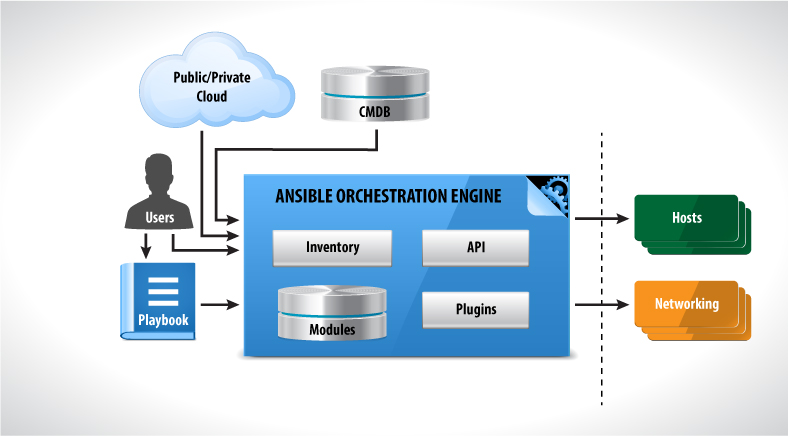
\includegraphics[width=\textwidth]{images/ansible_architect.jpg}}
    \end{center}
    \caption{Kiến trúc hệ thống của Ansible}
    \label{fig:ansible_arch}
\end{figure}

\newpage
\clearpage

Một trong những khác biệt chính giữa Ansible với những sản phẩm cùng loại chính là kiến trúc của nó

\begin{itemize}
\item Mặc định, Ansible quản lý các máy trạm thông qua giao thức SSH. Nó sử dụng một thư viện được gọi là \textbf{paramiko} (được viết bằng lập trình Python\footnote{\url{https://en.wikipedia.org/wiki/Python_(programming_language)}}) hoặc sử dụng ngay OpenSSH của hệ điều hành.

\item Ansible có thể truyền tải theo khác nhau, các phương thức là có thể thay đổi được. Ví dụ: Mặc dù \textbf{0mq} - một phương thức truyền tải tăng tốc (accelerated transport) được đưa ra nhưng Ansible hỗ trợ cả phương thức không sử dụng mạng.

\item Ansible không yêu cầu quyền root\footnote{account có quyền tuyệt đối với hệ thống trên Linux, BSD hay Solaris} để truy cập mà nó có thể cấu hình để dùng sudo\footnote{\url{https://en.wikipedia.org/wiki/Sudo}} trong các trường hợp cần thiết.

\item Ansible không yêu cầu một khóa SSH cụ thể hay một người dùng riêng. Nó có thể làm việc với bất cứ người sử dụng được cung cấp, nghĩa là Ansible tôn trọng quyền truy cập của hệ điều hành của bạn.

\item Khi có yêu cầu, Ansible sẽ chuyển các module cần thiết tới các nút điều khiển, sau đó chạy chúng từ xa với các thông tin người dùng đã được cung cấp và không để lại được bất cứ cài đặt gì trên các nút này.

\item Ansible không yêu cầu bất kỳ phần mềm máy chủ được chạy từ một máy quản lý, nó chỉ yêu cầu các thông tin đăng nhập của người dùng mà thôi.

\item Ansible không yêu cầu bất kì một phần mềm agent nào được chạy trên cái nút điều khiển.

\item Ansible không cần mở thêm bất cứ một cổng nào ngoài SSH cũng như không yêu cầu phải có hạ tầng PKI để bảo trì.

\item Những người có quyền truy cập vào máy chủ điều khiển (hoặc máy chủ điều khiển mã nguồn) không thể xóa hay thay đổi các nội dung các máy trạm (hoặc ra lệnh cho chúng chạy một lệnh nào đó) mà không có cũng có thông tin về hệ thống đó.

\item Khi không còn quản lý nữa, Ansible không dùng đến bất cứ tài nguyên nào của những máy trạm.

\end{itemize}

Những đặc điểm trên kết hợp với nhau làm cho Ansible trở nên lý tưởng cho các môi trường bảo mật hoặc hiệu suất cao, nơi có những lo ngại về sự ổn định hoặc việc thay đổi thường xuyên của các agent. Những thuộc tính trên hầu hết đều hữu ích trong các lĩnh vực về máy tính.

Ansible là sự thiết kế đồng nhất giữa kinh nghiệm của sử dụng và phương pháp tiếp cận. Ansible được thiết kế để làm cho việc cấu hình và xử lý các hạ tầng CNTT cũng chỉ đơn giản như việc đọc hoặc viết cấu hình, thậm chí đối với những người chưa qua đào tạo về việc đọc chúng.

Mặc dù Ansible có thể thực hiện hầu hết các loại nhiệm vụ tự động hóa, Ansible không giống với ngôn ngữ lập trình phần mềm, nó chỉ là các mô tả cơ bản về trạng và tiến trình. Hơn nữa, nó cố gắng để giải quyết nhiều vấn đề chồng chéo của tự động hóa hệ thống từ một framework duy nhất với mục tiêu giảm thiểu thời gian và chi phí để học và hiểu cũng như gắn kết nhiều framework với nhau.

Với các phương pháp truyền thống khác, người dùng thường phải kết hợp nhiều công cụ với nhau có để bao quát hết những điều cơ bản trong quản lý hệ thống CNTT và cấu hình phần mềm, bao gồm:

\begin{itemize}
\item Một công cụ dùng quản lý cấu hình, nó dùng để làm việc với các hệ điều hành cơ bản, mô tả các trạng thái mong muốn của một hệ thống, nhưng không phải quá trình để đưa nó vào trạng thái đó.

\item Một công cụ triển khai, dùng để đưa sản phẩm phần mềm lên hệ thống, nó tập trung vào quá trình thực hiện.

\item Một công cụ dùng để thực thi, cho các tác vụ thực thi tức thời - những thứ mà không phù hợp với mô hình trước đây, chẳng hạn như restart hàng loạt các máy chủ.
\end{itemize}

Ansible đã gộp tất cả các yếu tó đó thành một công cụ duy nhất, đồng thời cung cấp các khả năng và đặc điểm cho phép thực hiện triển khai những phần mềm nhiều lớp và các quy trình làm việc phức tạp.

\subsection{Mô hình sắp xếp công việc}

Để có thể hiểu được mô hình sắp xếp công việc (Modeling Orchestration Workflows) của Ansible, chúng ta lấy xem xét một ví dụ cụ thể về một ứng dụng web 3 lớp truyền thống bao gồm các thành phần:

\begin{itemize}
\item Các máy chủ ứng dụng
\item Các máy chủ cơ sở dữ liệu
\item Các máy chủ nội dung
\item Hệ thống cân bằng tải
\item Hệ thống giám sát được kết nối với hệ thống cảnh báo như một dịch vụ thông báo
\item Một hệ thống tích hợp liên tục\footnote{Continuous integration: \url{https://en.wikipedia.org/wiki/Continuous_integration}}
\end{itemize}

Theo như ví dụ trên, Ansible có thể xử lý một cách đơn giản theo mô hình như sau:

\begin{enumerate}
\item Tư vấn cách cấu hình và cài đặt kho chứa cho thông tin về các máy chủ tham gia.
\item Cấu hình hệ điều hành cơ sở trên tất cả các máy và thực hiện các công việc sao cho tất cả chúng có cùng một trạng thái mong muốn.
\item Xác định thành phần của các máy chủ ứng dụng web để cập nhật.
\item Đưa ra tín hiệu báo cho hệ thống giám sát chuyển các servers vào trạng thái offline.
\item Đưa ra tín hiệu báo cho hệ thống cân bằng tải tách các máy chủ ứng dụng ra khỏi hệ thống
\item Triển khai và cập nhật các máy chủ ứng dụng web
\item Đưa ra tín hiệu báo cho hệ thống cân bằng tải đưa các máy chủ ứng dụng này trở lại hệ thống.
\item Đưa ra tín hiệu báo cho hệ thống giám sát tiếp tục giám sát các sự cố trên các máy chủ này.
\item Lặp đi lặp lại quá trình này cho tới khi tất cả các máy chủ ứng dụng còn lại được cập nhật.
\item Lặp lại các quá trình cập nhật lần lượt này cho các lớp khác như máy chủ cơ sở dữ liệu hay máy chủ nội dung.
\item Gửi thư điện thử thông báo và giải trình khi quá trình cập nhật hoàn thành.
\end{enumerate}

\subsection{Các thành phần chính}

\textbf{\large Modules}
\addcontentsline{toc}{paragraph}{Modules}


Các module của Ansible là nguồn tài nguyên được phân phối cho các nút ở xa để yêu cầu chúng thực hiện một số nhiệm vụ hoặc đưa nút đó một vào một trạng thái thích hợp theo yêu cầu. Ansbile luôn đi theo triết lý "batteries included", vì vậy chúng ta có rất nhiều module tuyệt vời dành cho hầu hết các công việc lõi của ngành CNTT. Điều này có nghĩa là những module này luôn được cập nhật và chúng ta không cần phải cố gắng tìm kiếm cách để cho nó làm việc trên nền tảng của chúng ta. Chúng ta có thể tưởng tượng những module này là các thành phần của một bộ công cụ hữu ích với các công cụ quản lý hệ thống và các playbooks như một hướng dẫn để xây dựng một hệ thống bằng những công cụ này.

Với một số lượng khá lớn module, Ansible có khả năng dễ dàng triển khai những workloads tới một loạt các công nghệ ảo hóa và các dịch điện toán đám mây công cộng hay trên các môi trường tiền điện toán đám mây như VMware, OpenStack, Amazon Web Services EC2 (AWS), Eucalyptus Cloud, KVM, và CloudStack. Những máy chủ có thể được triển khai từ hình ảnh hệ điều hành cơ sở mà không có bất kỳ sửa đổi, đồng thời được cấu hình đầy đủ chỉ trong một bước.

Không chỉ vậy, hiện nay Ansible được sử dụng rộng rãi trong việc triển khai các hệ thống BigData, các hệ thống lưu trữ và phân tích môi trường bao gồm những nền tảng quan trọng như Hadoop, Riak, và Aerospike.

Trong những môi trường có nhiều máy chủ chưa được cấu hình nhưng chúng phải được cấu hình trước mà không cần bất kì một chương trình agent quản lý. Khách hàng yêu cầu một công cụ điều khiển đơn giản và dễ dàng chỉnh sửa các chính sách cho cả hai việc triển khai và cập nhật các cụm clusters.

Các khu vực khác bên ngoài lĩnh vực BigData cũng có thể tận dụng lợi thế này. Các tính chất này cũng làm cho Ansible hấp dẫn cho hệ thống giám sát lưu lượng truy cập cao tổ chức, nơi Ansible trả lại tất cả tài nguyên CPU có sẵn cho các môi trường máy tính khi không sử dụng. Không có việc lãng phí tài nguyên bộ nhớ hoặc CPU, cũng không cần phải có một daemon để duy trì hoạt động.

Để có thể tìm hiểu chi tiết hơn về chức năng của các module này trong Ansbile, chúng ta có thể tham khảo trang tài liệu của Ansbile Works. Tại địa chỉ \url{http://www.ansibleworks.com/docs/modules.html}

\textbf{\large Plugins}
\addcontentsline{toc}{paragraph}{Plugins}


Có rất nhiều điểm tích hợp có thể được sử dụng để mở rộng Ansible, bao gồm:

\begin{itemize}
\item Những module có thể chạy cục bộ hoặc từ xa để cấu hình các ứng dụng, các dịch vụ hoặc các tham số cho hệ điều hành.
\item Các phương thức mới ghi nhập các callback cho các chương trình kiểm soát hoặc báo cáo
\item Tích hợp với các nguồn dữ liệu bên ngoài
\item Các thông tin dữ liệu của Inventory từ hệ thống CMDB hoặc đám mây
\item Các phương thức chuyển vận mới mà từ đó Ansbile có thể giao tiếp với các máy mà mình quản lý
\end{itemize}

Cac đơn vị công việc trong ansbile được đảm bảo bởi các module, đó là những chương trình nhỏ chạy trên máy chủ ở xa để đảm bảo rằng máy chủ đó được đưa vào trạng thái chỉ định phù hợp. Các module này có thể viết bằng ngôn ngữ bất kì chẳng hạn như Python, Perl, Ruby hay bash script. Vì vậy, người dùng có thể sử dụng công cụ yêu thích của họ để tạo ra các module cho bản thân mình hay những người khác.

Mặc định, các module lõi đã được tạo sẵn, có nghĩa là chúng giúp hệ thống có được một trạng thái mong muốn, và nếu không có thay đổi trạng thái được thực hiện, chúng không làm gì ảnh hưởng tới hệ thống cả. Ansible cũng làm cho nó trở nên dễ dàng để mô hình hóa các quá trình được không tạo sẵn, và cũng làm cho nó có thể chỉ đơn giản là chỉ cần đẩy ra kịch bản đơn giản và chạy chúng như mong muốn. Sử dụng các module có sẵn là thích hơn, tuy nhiên, nhưng điều quan trọng là để có thể để mô hình bất kỳ loại quá trình nào chứ không chỉ một mà rơi vào những giới hạn của chúng. Ansible luôn thực tế trong vấn đề này.


\textbf{\large Playbooks}
\addcontentsline{toc}{paragraph}{Playbooks}


Trong Ansible, mọi công việc từ cấu hình hệ điều hành cơ sở đến mô hình hóa quá trình cập nhật hay thực thi ngay lập tức các công việc trên một máy chủ ở xa đều sử dụng chung một công cụ. Những cấu hình cụ thể được viết ra trong Ansible được gọi là "Playbooks". Đó một dạng mã mà cả con người và máy tính đều có thể phân tích được (một dạng mã YAML\footnote{\url{http://www.ansibleworks.com/docs/YAMLSyntax.html}}), đồng thời làm cho việc hợp tác với những chương trình khác dễ dàng hơn. Và quan trọng nhất là dễ đọc và hiểu đối với cả những người không phải là nhà phát triển.

Playbooks làm cho việc cấu hình hệ thống hay triển khai hệ thống trên nhiều máy trở lên đơn giản hơn bất kỳ công cụ nào đã có. Playbooks rất phù hợp trong việc triển khai các ứng dụng phức tạp.

Playbooks có thể khai báo cấu hình, nhưng nó cũng có thể dàn xếp các bước bất kì của một quá trình thủ công, thậm chí là cả những bước khác nhau khi mà chúng phải nhảy qua nhảy lại giữa một tập hợp các máy chủ với các nhiệm vụ khác nhau. Playbooks có thể thực hiện các công việc một cách đồng bộ hoặc không đồng bộ.

Trong khi bạn có thể chạy chính ansible cho các nhiệm vụ đột xuất, playbooks có thể được giữ trong các hệ thống kiểm soát mã nguồn và được sử dụng để đẩy đi các cấu hình hoặc đảm bảo cấu hình của hệ thống từ xa được giữ trong spec của nó.

Playbooks được thể hiện trong định dạng YAML với cú pháp được tối thiểu hóa. Những nhà phát triển Ansible đã hết sức cố gắng để làm cho nó không giống một ngôn ngữ lập trình hay script mà là giống một dạng mô hình cấu hình hay một quá trình.

Mỗi playbooks bao gồm một hay nhiều \textbf{play} trong danh sách

Mục tiêu của mỗi play là ánh xạ một nhóm các máy chủ với một số vai trò xác định, đại điện cho những điều mà Ansible gọi là nhiệm vụ (tasks). Ở mức độ cơ bản, một nhiệm vụ không gì hơn là gọi đến một module của Ansible

Bằng cách gộp nhiều plays, Playbooks có thể dàn xếp việc triển khai trên nhiều máy, chạy một số bước nhất định trên nhóm máy chủ web, sau đó một số khác trên nhóm máy cơ sở dữ liệu, sau đó lại là một nhóm lệnh khác trên các máy chủ web ... cứ vậy cho đến khi hoàn thành.

"plays" ít hoặc nhiều có những nét tương đồng với những môn thể thao. Chúng ta có có thể có khá nhiều plays ảnh hưởng đến hệ thống của chúng ta theo nhiều cách khác nhau. Điều đó nghĩa là nếu chúng ta định nghĩa ra một mô hình hoặc một trạng thái, chúng ta có thể chạy nhiều plays khác nhau tại các thời điểm khác nhau.

Dưới đây là một ví dụ về một playbooks chỉ chứa 1 plays:

\begin{lstlisting}[label={lst:ansbile_playbook_example},caption={Ví dụ về playbooks của Ansible},morekeywords={hosts, vars, tasks, name, yum, http_port, max_clients, remote_user, template, service, handlers, notify, state, pkg, src, dest}]
- hosts: webservers
  vars:
    http_port: 80
    max_clients: 200
  remote_user: root
  tasks:
  - name: ensure apache is at the latest version
    yum: pkg=httpd state=latest
  - name: write the apache config file
    template: src=/srv/httpd.j2 dest=/etc/httpd.conf
    notify:
    - restart apache
  - name: ensure apache is running
    service: name=httpd state=started
  handlers:
    - name: restart apache
      service: name=httpd state=restarted
\end{lstlisting}

Trong playbooks trên, chúng ta khai báo một cụm \textbf{webservers} ở cổng 80 và có số client tối đa là 200, sử dụng user root để điều khiển. Playbooks cũng thiết lập một số công việc và trạng thái mong muốn với nó:

\begin{itemize}
\item Đảm bảo chắc chắn rằng Apache httpd server là phiên bản mới nhất
\item Đảm bảo config của Apache \textbf{/etc/httpd.conf} giống như template có sẵn ở \textbf{/srv/httpd.j2}. Đồng thời thiết lập thông báo khi Apache restart.
\item Đảm bảo rằng Apache đã được khởi động
\end{itemize}



\newpage
\clearpage
\section*{Tổng kết}

\newpage
\chapter{Triển khai thực nghiệm}
\section{Bài toán}
\section{Phân tích}
\section{Triển khai}

\backmatter
\pagestyle{empty}
\chapter*{Kết luận}
\addcontentsline{toc}{chapter}{Kết luận}

Tự động hóa hệ thống tuy không phải một vấn đề mới nhưng luôn là vấn đề đau đầu của những người quản trị hệ thống. Nhưng không giống như trước kia, ngày nay, chúng ta có thể sử dụng rất nhiều các công cụ để làm việc đó thay vì phải làm thủ công bằng các kịch bản truyền thống. Puppet, Chef hay Ansible là những công cụ cực kì hữu dụng mà bất cứ một nhà quản trị hệ thống nào hiện nay đều nên biết và sử dụng chúng trong công việc của mình.

Những kết quả của nghiên cứu này có thể là chưa sâu và bao quát hết được các tính năng của các công cụ đã giới thiệu. Nhưng đồ án này mang lại cái nhìn tổng quan và bao quát cho những ai chưa từng tiếp xúc với tự động hóa hệ thống, để họ có thể hiểu và áp dụng được nó vào thực tế công việc của từng người.

Người viết đồ án với mục đích là nghiên cứu để có thể triển khai trên thực tế các hoạt động tự động hóa cho hạ tầng các sản phẩm công nghệ đã học hỏi và rút ra được một số những kinh nghiệm quý cho bản thân. Trong tương lai, người viết sẽ cố gắng để hiểu sâu và thử nghiệm nhiều hơn nữa các công cụ này trong công việc hiện tại, nhằm nâng cao hiệu quả công việc của bản thân cũng như đồng nghiệp.



\newpage
\begin{thebibliography}{9}
\addcontentsline{toc}{chapter}{Tài liệu tham khảo}
\bibitem{} James Turnbull and Jeffrey McCune, \emph{"Pro Puppet"}, Apress, pp. 1-5, May 2011.
\bibitem{} Amy Brown and Greg Wilson, \emph{"The Architecture Of Open Source Applications, Volume II"}, Lulu.com, pp. 309-322, May 2008.
\bibitem{} Grace Walker, \emph{"Cloud computing fundamentals - A different way to deliver computer resources"}, IBM developerWorks, December 2010.
\bibitem{} Peter Mell and Timothy Grance, \emph{"The NIST Definition of Cloud Computing"}, NIST Special Publication 800-145, Apr 2012.
\bibitem{} Puppet Labs, \emph{"Puppet Labs Documentation"}, \\URL: \url{http://docs.puppetlabs.com/}
\bibitem{} Opscode, \emph{"Chef Documents"}, \\URL: \url{http://docs.opscode.com/}
\bibitem{} Ansible Works, \emph{"Ansible Documents"}, \\URL: \url{http://www.ansibleworks.com/docs/}
\end{thebibliography}

\centerline{\bf \large\MakeUppercase{Hết}}

\end{document}